%% LyX 2.0.2 created this file.  For more info, see http://www.lyx.org/.
%% Do not edit unless you really know what you are doing.
\documentclass[english,noae]{article}
\usepackage[T1]{fontenc}
\usepackage{amsmath}
\usepackage{amssymb}

\makeatletter

%%%%%%%%%%%%%%%%%%%%%%%%%%%%%% LyX specific LaTeX commands.
%% Because html converters don't know tabularnewline
\providecommand{\tabularnewline}{\\}

%%%%%%%%%%%%%%%%%%%%%%%%%%%%%% Textclass specific LaTeX commands.

\makeatother

\usepackage{babel}
\usepackage{Sweave}
\begin{document}
\Sconcordance{concordance:dizzysNewInfec.tex:dizzysNewInfec.Rnw:%
1 167 1 1 2 1 0 1 5 4 0 1 3 5 0 1 2 1 1 1 2 1 0 1 1 4 0 1 2 6 1 1 3 2 0 %
1 1 4 0 1 2 1 1 1 2 1 0 1 1 4 0 1 2 1 1 1 2 1 0 1 1 4 0 1 2 3 1 1 2 1 0 %
1 1 4 0 1 2 1 1 1 5 4 0 1 1 1 4 2 0 1 1 4 0 1 2 16 1}


\title{$\mathbf{dizzys}$: efficient deterministic/stochastic simulations
in R for a metapopulation by using SIR/SEIR models}


\author{TRAN Thi Cam Giang}
\maketitle
\begin{abstract}
Predicting the potential spread of an infectious disease is still
a difficult problem for scientists. It requires much more than simple
connecting subpopulations in a metapopulation and takes into account
many factors about the pathogen and the affected subpopulation. Therefore,
this 'dizzysNewInfec' package allows us to simulate dynamics of an infectious
disease through subpopulations by using the SIR/SEIR models and by
implementing the direct algorithm of Gillespie in 1977 and the adaptive
tau leaping to approximate the trajectory of a continuous-time stochastic
process. Consequently, result returned is biological data in time
horizon about the disease dynamic, we can perform analysis on this
biological data. This vignette presents a few examples of SIR/SEIR
applied to biological problems. 
\end{abstract}

\section*{Introduction}

Fundamentally, Kermack-McKendrick gave the first epidemic model to
provide a mathematical description of the kinetic transmission of
an infectious disease in an unstructured subpopulation. According
to this model, today we have known well the SIR/SEIR deterministic epidemic
models. This is the two basic models very popularly used by scientists.
However, Keeling2008 \cite{KeelingRohani2008} show that all the deterministic
models are essentially fixed "clockwork" systems with the same
starting conditions, exactly the same trajectory is always observed.
It isn't right for dynamics of real pathogens in the real-world. So
stochastic models are created and concerned with approximating or
mimicking the random or probabilistic element from the deterministic
models. Moreover, when the quantities in a system are small enough
and extinction is probable to occur, then stochastic effects become
critical to take into account. This is reason, in the 'dizzysNewInfec' package,
it permits us to obtain the dynamics of the deterministic and the
approximate dynamics of the stochastic epidemic models.

Based on the stochastic models, their processes are in Markov process,
it means that the future state of the process, conditional on the
present state, is independent of the past. In the case, our package
focus on simulating dynamics from a continuous-time Markov process
for which the transition rates are constants, isn't a function of
time. We use the exact algorithm of Gillespie in 1977 and the approximate
algorithm described as the "adaptive tau-leaping algorithm". With
these two algorithms, each has its private advantages and its private
disadvantages. For the exact algorithm, it give us a really exact
approach of simulating population-based time-to-event through two
step with many iterations of 1) searching the time of next event by
an exponentially distributed function and 2) searching the nature
of next event. This Gillespie's solution becomes too slow and impractical
as any one transition rate grows large. Hence, approximate models
are born instead of the Gillespie's solution, they are concerned with
larger transition rates and with increasing simulation speed while
still maintaining reasonable accuracy. The "adaptive tau-leaping
algorithm" known as an approximate method reduces the number of
iterations by treating transition rates as constant over time periods
for which this approximation leads to little error\cite{Cao2007}. 

The \textbf{dizzysNewYann} package in R implements both the exact solution
and the approximate solution for the SIR and SEIR models by integrating
the R package and the C++ implementation. We can choose one of the
two solutions to simulate when the number of subpopulations in a metapopulation
increases. We use C++ to perform the algorithms, and R to create interfaces. Therefore, new implementation is much
faster than any pure R implementation.


\section*{Methods}

In this section, first we will talk about the deterministic model,
the stochastic model of the SEIR model. Then, we will have transformation
the SEIR model into the SIR model through the usage of the two algorithms.
We hope that the models and the algorithms should be well understood
before obtainning simulation results.


\subsection*{Deterministic model:}

To describe infectious diseases in a in a spatial context, we consider
a metapopulation of n sub-populations. In subpopulation $i$ of size
$N_{i}$, disease dynamics can be deterministically described by the
following set of differential equations: 
\begin{eqnarray}
\frac{dS_{i}}{dt} & = & \mu N_{i}-\lambda_{i}S_{i}-\mu S_{i}\label{eq:dS-1}\\
\frac{dE_{i}}{dt} & = & \lambda_{i}S_{i}-\mu E_{i}-\sigma E_{i}\\
\frac{dI_{i}}{dt} & = & \sigma E_{i}-\mu I_{i}-\gamma I_{i}\label{eq:infectieux-1}\\
\frac{dR_{i}}{dt} & = & \gamma I_{i}-\mu R_{i}\label{eq:dR-1}
\end{eqnarray}
 where $S_{i}$, $E_{i}$, $I_{i}$ et $R_{i}$ are respectively the
numbers of susceptible, exposed, infectious and recovered in this
sub-population $i$. Individuals are born susceptible and die at a
rate $\mu$, become infected with the force of infection $\lambda_{i}$,
infectious after a latency period of an average duration of $1/\sigma$
and recover at the rate $\gamma$. In case the infectious contact
rate is constant, the equilibrium values of the variables $S$, $E$,
$I$ and $R$ can be expressed analytically (see appendix). The force
of infection depends not only on the total population size $N_{i}$
and the number of infected $I_{i}$ in subpopulation $i$, but also
in other sub-populations : 

\begin{equation}
\lambda_{i}=\sum_{j}\rho_{ij}\kappa_{j}\log\left[1-\sum_{k=1}^{M}\left(\frac{\left|I_{k,t}\right|}{N_{k}}\times c_{ik}\times\xi_{jk}\right)\right]
\end{equation}

where 
$\rho_{i,j}$ the probability that an individual from subpopulation $i$ visits subpopulation $j$.
$\kappa_{j}$ is the average number of contacts per unit of time a susceptible will have when visiting city.
$c_{i,k}$ is the probability that a susceptible individual native from $i$ being in contact with another infected individual native from 
$k$.
$\xi_{jk}$ refers to the probability that an individual $y$ meeting $x$ in  $C_{j}$ comes from  $C_{k}$.


See appendix for detail on the construction of this equation.
We can verify that in the limit case on one single subpopulation in
the metapopulation ($i=j$ et $n=1$) we have 

\begin{equation}
\lambda_{i}=\rho_{ii}*\kappa_{i}*\log\left[1-(\frac{\left|I_{i,t}\right|}{N_{i}}\times c_{ik}\times\xi_{jk}\right)\right]
\end{equation}
 consider that the contact number $\rho_{ii}$ is seasonally forced
\cite{Altizer2006}: 
\begin{equation}
\beta_{i}(t)=b_{0}\left[1+b_{1}\cos\left(\frac{2\pi t}{T}+\varphi_{i}\right)\right]\label{eq:beta_i-1}
\end{equation}
 where $b_{0}$ and $b_{1}$ are the mean value and amplitude of the
contact rate and $T$ and $\varphi_{i}$ are the period and the phase
of the forcing.


\subsection*{Stochastic model using Gillespie's exact algorithm:}

Based on the differential equations above, we give a stochastic version
of this model. We use for that a population-based time-to-next-event
model based on Gillespie's algorithm \cite{Daniel.T.Gillespie1977}.
Table \ref{tab:stoch_ev} lists all the events of the model, occurring
in subpopulation $i$. 
\begin{table}[htpb]
\begin{centering}
\caption{\label{tab:stoch_ev}Events of the stochastic version of the model
of equations \ref{eq:dS-1}-\ref{eq:dR-1}, occuring in subpopulation
$i$.}

\par\end{centering}

\centering{}\textbf{}%
\begin{tabular}{lcc}
\textbf{Events } & \textbf{Rates } & \textbf{Transitions }\tabularnewline
\textbf{birth}  & $\mu N_{i}$  & $S_{i}\leftarrow S_{i}+1$ and $N_{i}\leftarrow N_{i}+1$ \tabularnewline
\textbf{death of a susceptible } & \textbf{$\mu S_{i}$ } & \textbf{$S_{i}\leftarrow S_{i}-1$ }\tabularnewline
\textbf{death of an exposed } & \textbf{$\mu E_{i}$ } & \textbf{$E_{i}\leftarrow E_{i}-1$ }\tabularnewline
\textbf{death of an infected } & \textbf{$\mu I_{i}$ } & \textbf{$I_{i}\leftarrow I_{i}-1$ }\tabularnewline
\textbf{death of an immune } & \textbf{$\mu R_{i}$ } & \textbf{$I_{i}\leftarrow I_{i}-1$ }\tabularnewline
\textbf{infection } & \textbf{$\lambda_{i}S_{i}$ } & \textbf{$S_{i}\leftarrow S_{i}-1$ }and\textbf{ $E_{i}\leftarrow E_{i}+1$ }\tabularnewline
\textbf{becoming infectious } & \textbf{$\sigma E_{i}$ } & \textbf{$E_{i}\leftarrow E_{i}-1$ }and\textbf{ $I_{i}\leftarrow I_{i}+1$ }\tabularnewline
\textbf{recovery } & \textbf{$\gamma I_{i}$ } & \textbf{$I_{i}\leftarrow I_{i}-1$ }and\textbf{ $R_{i}\leftarrow R_{i}+1$ }\tabularnewline
 &  & \tabularnewline
\end{tabular}
\end{table}



\subsection*{Stochastic model using ``adaptive tau-leaping algorithm'':}

In this step, we provide basic concepts for the adaptive tau-leaping
algorithm by using the detailed description of Cao\cite{Cao2007}. 

For the Markov process at time t, to describe a metapopulation of
n subpopulations, we have:

\textbf{state set:} X(t)

$X(t):=[S_{1}(t),S_{2}(t),...,S_{n}(t),E_{1}(t),E_{2}(t),...,E_{n}(t),I_{1}(t),I_{2}(t),...,I_{n}(t),R_{1}(t),R_{2}(t),...,R_{n}(t)]$

each variables of $X(t)$ is defined on the non-negative integers. 

\textbf{set of allowable transitions:} ${\triangle_{j}}$, for each
allowable transition, $j$, we define a rate $\lambda_{j}$, by using
a function independent on t but dependent on the current state $X(t)$,
to calculate transition rates given the state $(\lambda(X))$ through
the deterministic model, and a vector of $n$ integers, $\triangle_{j}:=[\triangle_{j,1},...,\triangle_{j,n}]$,
that reflects the change in state if this transition were followed:
$X(t)+\triangle_{j}$. 

\textbf{time process: }modeling on a time-homogeneous process.

\textbf{operation:} with the SEIR model, the package simulates a trajectory
from time $0$ to a stopping time $tmax$. Based on the description
of Cao and al.{[}2007{]}, a good time period of length $\tau$ is
during which all transition rates remain approximately constant and
all $n$ state variables remain greater than zero with probability$\thicksim1$.
Then, by using the Poisson-dustributed number of transitions, that
should have occurred during this period: $X(t+\tau)\approx X(t)+\sum_{j}y_{j}\triangle_{j}$
where $y_{j}\thicksim Poisson(\tau\lambda_{j})$. To successfully
apply this algorithm, we need to know that, transition rates frequently
change and in balancing efficiency with accuracy when selecting these
time periods to leap over.


\subsection*{Transformation SEIR model into SIR model:}

The SIR model used in this package is the SIR model with births and
death\textbf{. }By observing this SEIR model, if we give a numerical
value for the parameter $\sigma$ then a SEIR model would have. On
the other side, if we give $Inf$ (to infinity) the parameter $\sigma$
then we have a SIR model with birth and death (because, basically,
a SEIR model tends to a SIR model when $\sigma$ tends to infinity).


\section*{Example 1}

The deterministic SEIR model with one subpopulation by exploiting the 'seir' function in the package.

\begin{Schunk}
\begin{Sinput}
> library(dizzysNewInfec)
> # We have the values of parameters and of variables. 
> # Here, we have S=E=I=R=NULL and N=1e7.
> # It means that we use N=1e7 to calculate the equilibrium values of variables.
> obj<- globSEIRNewInfec(typeSIMU="deterministic",duration=5*365,mu=1/(70*365),sigma=1/8,gamma=1/5,
+ phiPHASE=0,nbVilles=1,S=NULL,E=NULL,I=NULL,R=NULL,N=1e7)
> # Use the plot function of the seir class
> plot(obj,col="red",ylab="number of infectives", xlab="time (day)") 
\end{Sinput}
\end{Schunk}
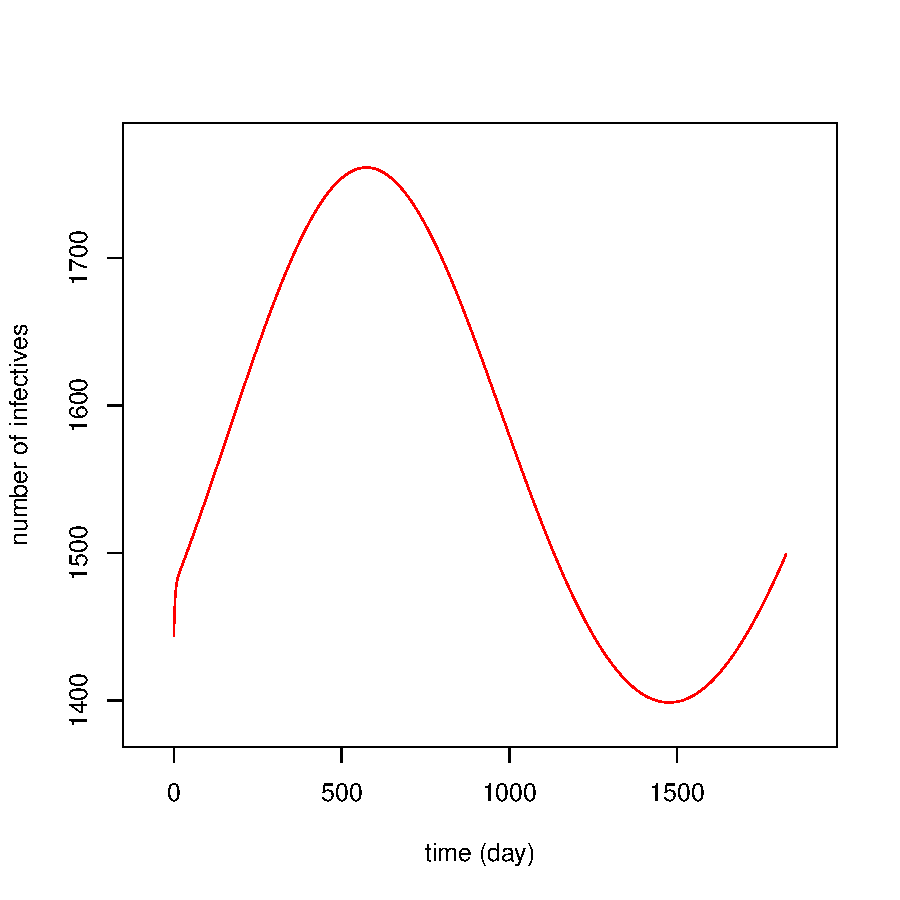
\includegraphics{dizzysNewInfec-002}

Now, we want to continue or to redo this simulation with other values of parameter, we can do it by exploiting the 'simul' function in the package.

\begin{Schunk}
\begin{Sinput}
> newobj<- globSEIRSimulNewInfec(obj,duration= 10*365,continue=T, append=T, nbCONTACT1=0.0, phiPHASE=pi/2)
> plot(newobj,col="red",ylab="number of infectives", xlab="time (day)") 
> 
\end{Sinput}
\end{Schunk}
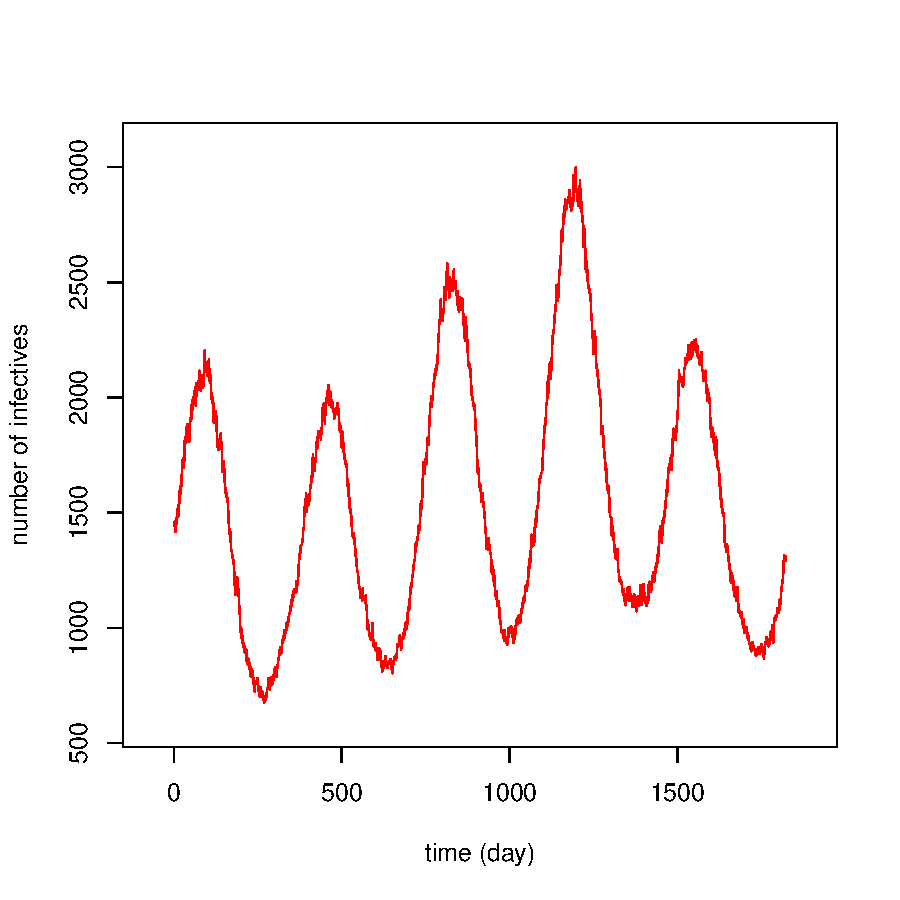
\includegraphics{dizzysNewInfec-003}

\section*{Example 2}

The SEIR stochastic model using Gillespie's algorithm by using the 'seir' function.

1) with one subpopulation:

\begin{Schunk}
\begin{Sinput}
> obj<- globSEIRNewInfec(typeSIMU="stochastic",method="direct",duration=5*365,mu=1/(70*365),sigma=1/8,gamma=1/5,phiPHASE=0,
+ nbVilles=1,S=NULL,E=NULL,I=NULL,R=NULL,N=1e7)
> plot(obj,col="red",ylab="number of infectives", xlab="time (day)") 
\end{Sinput}
\end{Schunk}
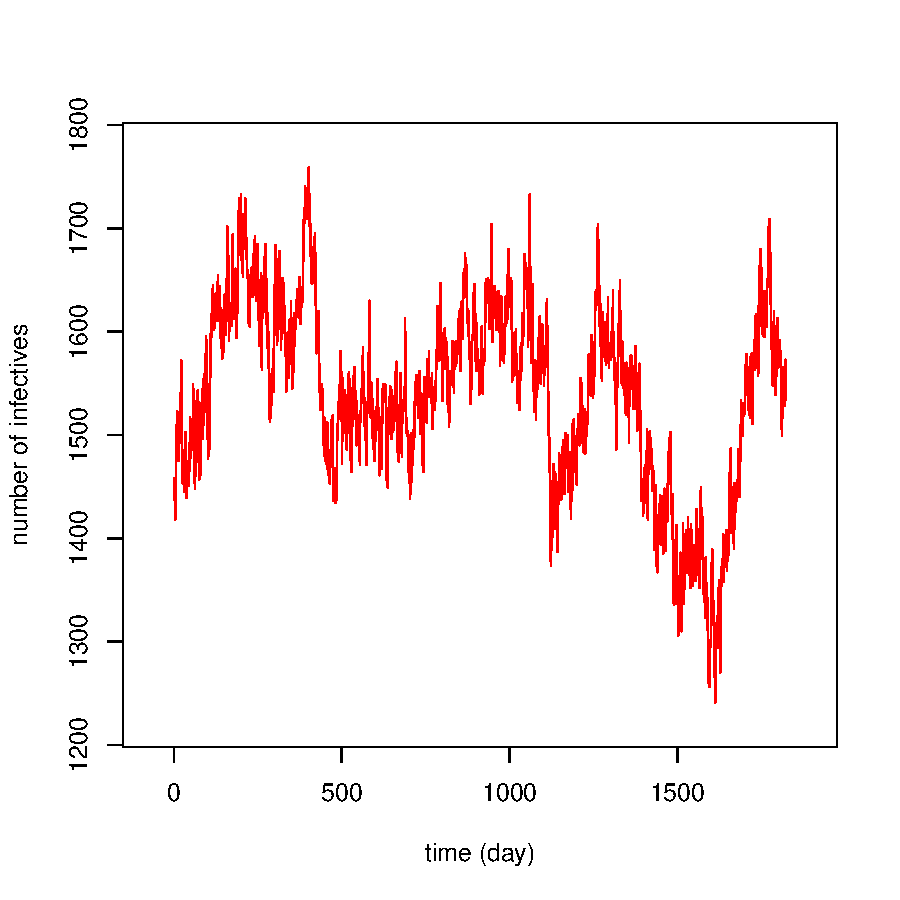
\includegraphics{dizzysNewInfec-004}

2) with three subpopulations and the different number of populations.

\begin{Schunk}
\begin{Sinput}
> obj<- globSEIRNewInfec(typeSIMU="stochastic",duration=5*365,mu=1/(70*365),sigma=1/8,gamma=1/5,nbVilles=3,N=c(1e7,1e6))
> plot(obj,col=c("red","blue"),ylab="number of infectives", xlab="time (day)") 
\end{Sinput}
\end{Schunk}
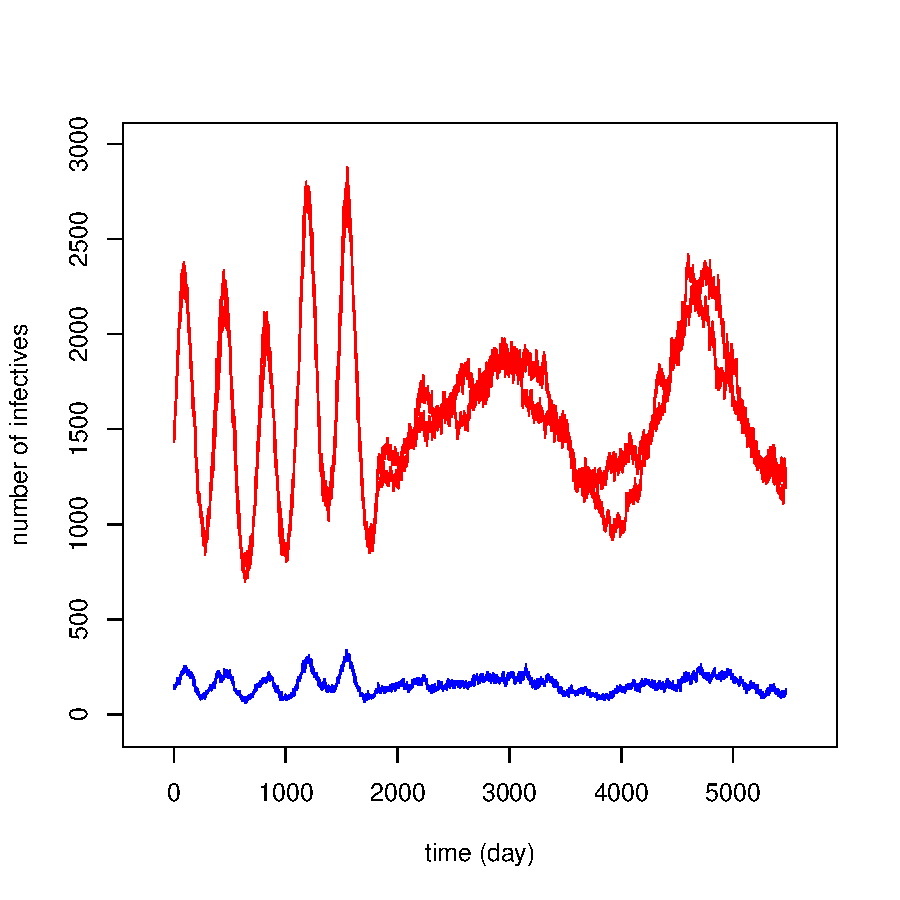
\includegraphics{dizzysNewInfec-005}

3) continue or redo this siluation with other values of parameter, we can do it by exploiting the 'simul' function in the package.
\begin{Schunk}
\begin{Sinput}
> newobj<- globSEIRSimulNewInfec(obj,duration= 10*365,typeSIMU="stoch",continue=T,append=T,nbCONTACT1=0.0,phiPHASE=pi/2)
> plot(newobj,col=c("red","blue"),ylab="number of infectives",xlab="time (day)")
> 
\end{Sinput}
\end{Schunk}
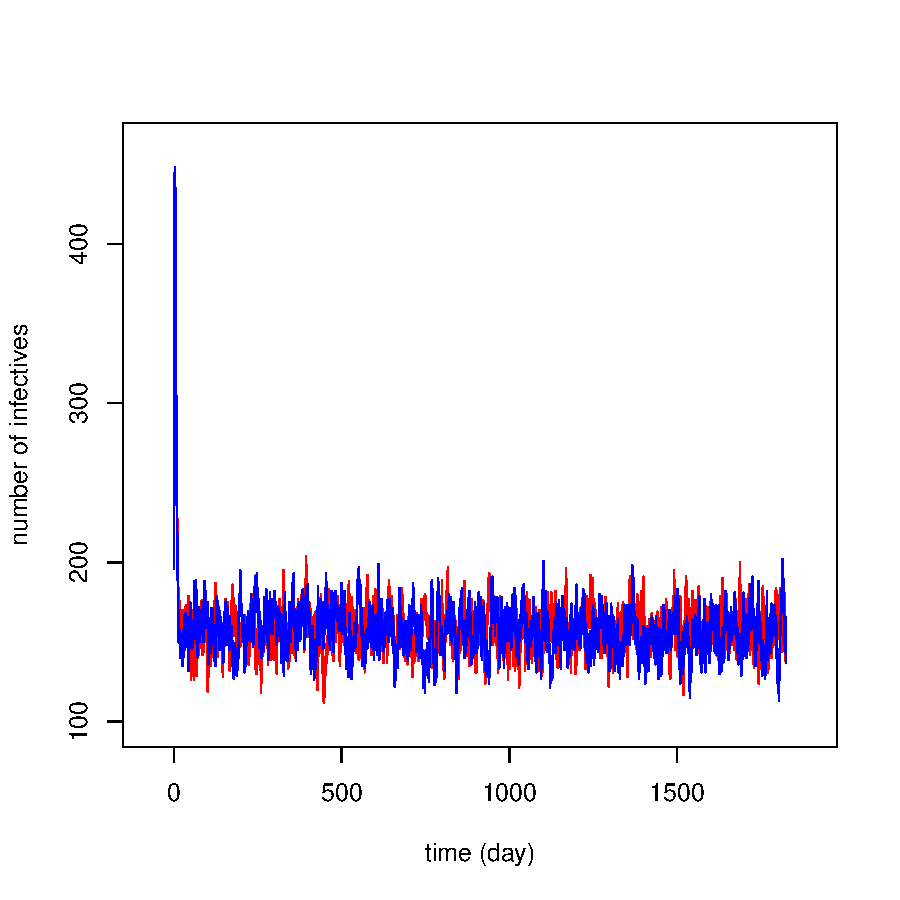
\includegraphics{dizzysNewInfec-006}

\section*{Example 3}

The SEIR stochastic model using "adaptive tau-leaping algorithm" by exploiting the 'seir' function. To do this algorithm, we only make the parameter method="adaptivetau" as follows: 

\begin{Schunk}
\begin{Sinput}
> obj<- globSEIRNewInfec(typeSIMU="stochastic",method="adaptivetau",duration=5*365,mu=1/(70*365),sigma=1/8,gamma=1/5,nbVilles=3,N=1e7)